% Auto-generated by experiments.analysis.generate_ci_plots --- do not edit.
\begin{figure}[H]
\centering
\adjustbox{max width=\textwidth}{%
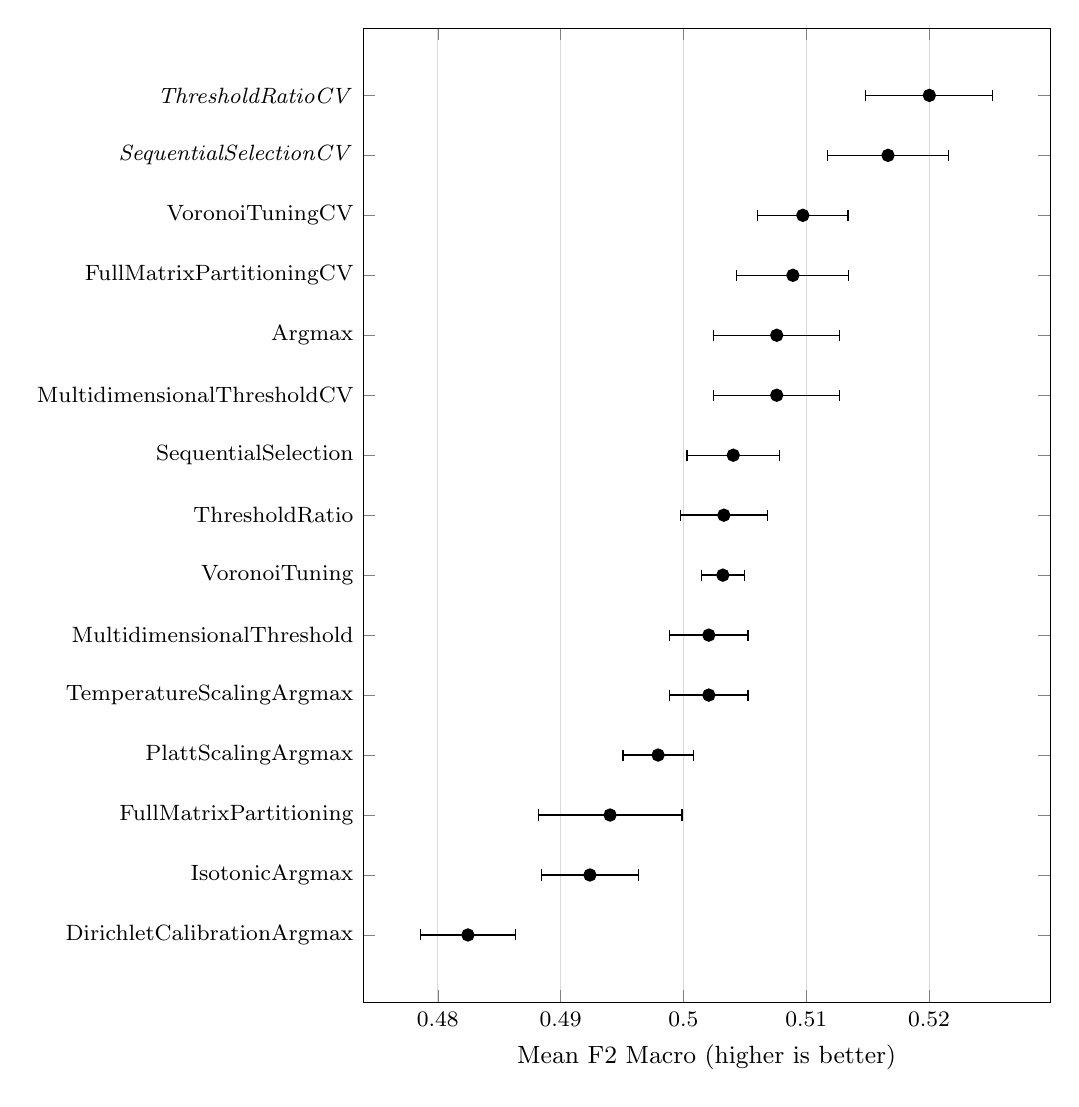
\begin{tikzpicture}
\begin{axis}[
    width=0.85\textwidth, height=13.95cm,
    xlabel={Mean F2 Macro (higher is better)},
    symbolic y coords={{ThresholdRatioCV},{SequentialSelectionCV},{VoronoiTuningCV},{FullMatrixPartitioningCV},{Argmax},{MultidimensionalThresholdCV},{SequentialSelection},{ThresholdRatio},{VoronoiTuning},{MultidimensionalThreshold},{TemperatureScalingArgmax},{PlattScalingArgmax},{FullMatrixPartitioning},{IsotonicArgmax},{DirichletCalibrationArgmax}},
    ytick={{ThresholdRatioCV},{SequentialSelectionCV},{VoronoiTuningCV},{FullMatrixPartitioningCV},{Argmax},{MultidimensionalThresholdCV},{SequentialSelection},{ThresholdRatio},{VoronoiTuning},{MultidimensionalThreshold},{TemperatureScalingArgmax},{PlattScalingArgmax},{FullMatrixPartitioning},{IsotonicArgmax},{DirichletCalibrationArgmax}},
    yticklabels={\textit{ThresholdRatioCV},\textit{SequentialSelectionCV},VoronoiTuningCV,FullMatrixPartitioningCV,Argmax,MultidimensionalThresholdCV,SequentialSelection,ThresholdRatio,VoronoiTuning,MultidimensionalThreshold,TemperatureScalingArgmax,PlattScalingArgmax,FullMatrixPartitioning,IsotonicArgmax,DirichletCalibrationArgmax},
    y dir=reverse,
    enlarge y limits=0.08,
    xmajorgrids=true,
    major grid style={draw=black!15, line width=0.3pt},
    scaled x ticks=false,
    xticklabel style={/pgf/number format/fixed, /pgf/number format/precision=3},
    tick label style={font=\footnotesize},
    label style={font=\small},
    every axis plot/.append style={thick},
]
\addplot[only marks, mark=*, mark size=2pt, color=black, error bars/x dir=both, error bars/x explicit, error bars/error bar style={color=black, line width=0.5pt}] coordinates { (0.520024,{ThresholdRatioCV}) +- (0.00517868,0) };
\addplot[only marks, mark=*, mark size=2pt, color=black, error bars/x dir=both, error bars/x explicit, error bars/error bar style={color=black, line width=0.5pt}] coordinates { (0.51666,{SequentialSelectionCV}) +- (0.00495574,0) };
\addplot[only marks, mark=*, mark size=2pt, color=black, error bars/x dir=both, error bars/x explicit, error bars/error bar style={color=black, line width=0.5pt}] coordinates { (0.509723,{VoronoiTuningCV}) +- (0.0036767,0) };
\addplot[only marks, mark=*, mark size=2pt, color=black, error bars/x dir=both, error bars/x explicit, error bars/error bar style={color=black, line width=0.5pt}] coordinates { (0.508913,{FullMatrixPartitioningCV}) +- (0.00455732,0) };
\addplot[only marks, mark=*, mark size=2pt, color=black, error bars/x dir=both, error bars/x explicit, error bars/error bar style={color=black, line width=0.5pt}] coordinates { (0.507598,{Argmax}) +- (0.00512521,0) };
\addplot[only marks, mark=*, mark size=2pt, color=black, error bars/x dir=both, error bars/x explicit, error bars/error bar style={color=black, line width=0.5pt}] coordinates { (0.507598,{MultidimensionalThresholdCV}) +- (0.00512521,0) };
\addplot[only marks, mark=*, mark size=2pt, color=black, error bars/x dir=both, error bars/x explicit, error bars/error bar style={color=black, line width=0.5pt}] coordinates { (0.504059,{SequentialSelection}) +- (0.00376794,0) };
\addplot[only marks, mark=*, mark size=2pt, color=black, error bars/x dir=both, error bars/x explicit, error bars/error bar style={color=black, line width=0.5pt}] coordinates { (0.503293,{ThresholdRatio}) +- (0.00352692,0) };
\addplot[only marks, mark=*, mark size=2pt, color=black, error bars/x dir=both, error bars/x explicit, error bars/error bar style={color=black, line width=0.5pt}] coordinates { (0.503212,{VoronoiTuning}) +- (0.00173639,0) };
\addplot[only marks, mark=*, mark size=2pt, color=black, error bars/x dir=both, error bars/x explicit, error bars/error bar style={color=black, line width=0.5pt}] coordinates { (0.502071,{MultidimensionalThreshold}) +- (0.00318547,0) };
\addplot[only marks, mark=*, mark size=2pt, color=black, error bars/x dir=both, error bars/x explicit, error bars/error bar style={color=black, line width=0.5pt}] coordinates { (0.502071,{TemperatureScalingArgmax}) +- (0.00318547,0) };
\addplot[only marks, mark=*, mark size=2pt, color=black, error bars/x dir=both, error bars/x explicit, error bars/error bar style={color=black, line width=0.5pt}] coordinates { (0.49794,{PlattScalingArgmax}) +- (0.00286004,0) };
\addplot[only marks, mark=*, mark size=2pt, color=black, error bars/x dir=both, error bars/x explicit, error bars/error bar style={color=black, line width=0.5pt}] coordinates { (0.494029,{FullMatrixPartitioning}) +- (0.00585333,0) };
\addplot[only marks, mark=*, mark size=2pt, color=black, error bars/x dir=both, error bars/x explicit, error bars/error bar style={color=black, line width=0.5pt}] coordinates { (0.492389,{IsotonicArgmax}) +- (0.00395195,0) };
\addplot[only marks, mark=*, mark size=2pt, color=black, error bars/x dir=both, error bars/x explicit, error bars/error bar style={color=black, line width=0.5pt}] coordinates { (0.482454,{DirichletCalibrationArgmax}) +- (0.00386869,0) };
\end{axis}
\end{tikzpicture}%
}
\caption{fot\_proving: F2 Macro on LGBM (higher is better). Each dot is a strategy's mean over ten seeds with a $\pm 1$ SE horizontal bar; rows are sorted by mean, and the best strategy and any whose interval overlaps it are italicized.}%
\label{fig:ci-fot_proving-f2_macro}
\end{figure}
